\documentclass[../main.tex]{subfiles}
\begin{document}
\appendix
\section{Code Snippets}
\begin{lstlisting}[language=C,caption="Camera settings"]
    camera cam;

    cam.aspectratio = 16.0f / 9.0f;
    cam.image_width = 1200;
    cam.samples_per_pixel = 10;
    cam.max_depth = 20;

    cam.fov = 20;
    cam.lookfrom = point3(13, 2, 3);
    cam.lookat = point3(0, 0, 0);
    cam.vup = Vec3(0, 1, 0);

    cam.background = color(0.7, 0.8, 1.0);

\end{lstlisting}
\begin{lstlisting}[language=C, caption="Generation of Rays", breaklines=true]
    Ray sendRay(int i, int j, int s_i, int s_j) {
        auto offset = sample_square_stratified(s_i, s_j);
        auto pixel_sample =
            pixel00_loc + ((float) (i) * pixel_delta_u) + ((float) (j) * pixel_delta_v);
    
        glm::vec3 ray_origin =
            (defocus_angle <= 0) ? center : defocus_disk_sample();
        glm::vec3 ray_direction = pixel_sample - ray_origin;
    
        return Ray(ray_origin, ray_direction);
      }    
\end{lstlisting}
\begin{lstlisting}[language=C, caption="BVH Node Structure", breaklines=true]
    class bvh_node : public Hittable {

    public:
      bvh_node(hittable_list &list)
          : bvh_node(list.objects, 0, list.objects.size()) {}
    
      bool hit(const Ray &r, float t_min, float t_max,
               hitrecord &rec) const override {
        if (!bbox.hit(r, interval(t_min, t_max)))
          return false;
    
        bool hit_left = left->hit(r, t_min, t_max, rec);
        bool hit_right = right->hit(r, t_min, hit_left ? rec.t : t_max, rec);
    
        return hit_left || hit_right;
      }
    
      aabb bounding_box() const { return bbox; }
    
      bvh_node(std::vector<shared_ptr<Hittable>> &objects, size_t start,
               size_t end);
    
    private:
      std::shared_ptr<Hittable> left;
      std::shared_ptr<Hittable> right;
      aabb bbox;
    
      static bool box_compare(const shared_ptr<Hittable> a,
                              const shared_ptr<Hittable> b, int axis) {
        auto a_axis_interval = a->bounding_box().axis_interval(axis);
        auto b_axis_interval = b->bounding_box().axis_interval(axis);
        return a_axis_interval.min < b_axis_interval.min;
      }
    
      static bool box_x_compare(const shared_ptr<Hittable> a,
                                const shared_ptr<Hittable> b) {
        return box_compare(a, b, 0);
      }
      static bool box_y_compare(const shared_ptr<Hittable> a,
                                const shared_ptr<Hittable> b) {
        return box_compare(a, b, 1);
      }
      static bool box_z_compare(const shared_ptr<Hittable> a,
                                const shared_ptr<Hittable> b) {
        return box_compare(a, b, 2);
      }
    };
    
    
\end{lstlisting}

\begin{lstlisting}[language=C, caption="Oct-Tree definition and implementation", breaklines=true]


class Octree
{
public:
    Octree(const aabb& boundingBox, int maxDepth = 15, int maxTrianglesPerNode = 100)
        : bbox(boundingBox), depth(0), maxDepth(maxDepth), maxTrianglesPerNode(maxTrianglesPerNode)
    {
    }

    void build(const std::vector<std::shared_ptr<Triangle>>& triangles, int depth = 0);

    bool hit(const Ray& r, float t_min, float t_max, hitrecord& rec) const;

private:
    void subdivide();

private:
    aabb bbox;
    int depth;
    int maxDepth;
    int maxTrianglesPerNode;

    std::vector<std::shared_ptr<Triangle>> triangles;
    std::unique_ptr<Octree> children[8];
};
void Octree::build(const std::vector<std::shared_ptr<Triangle> > &triangles, int depth) {
    this->depth = depth;

    if (triangles.size() <= maxTrianglesPerNode || depth >= maxDepth) {
        this->triangles = triangles;
        return;
    }

    subdivide();

    std::vector<std::shared_ptr<Triangle> > childrenTriangles[8];
    for (const auto &triangle: triangles) {
        aabb triangleBoundingBox = triangle->bounding_box();
        for (int i = 0; i < 8; i++) {
            if (children[i]->bbox.intersect(triangleBoundingBox)) {
                childrenTriangles[i].push_back(triangle);
            }
        }
    }

    // now recursively build the children
    for (int i = 0; i < 8; i++) {
        children[i]->build(childrenTriangles[i], depth + 1);
    }
}

void Octree::subdivide() {
    glm::vec3 center = bbox.center();
    glm::vec3 halfSize = bbox.half_size();

    children[0] = std::make_unique<Octree>(aabb(bbox.min(), center)); // Bottom-left-front
    children[1] = std::make_unique<Octree>(aabb(glm::vec3(center.x, bbox.min().y, bbox.min().z),
                                                glm::vec3(bbox.max().x, center.y, center.z))); // Bottom-right-front
    children[2] = std::make_unique<Octree>(aabb(glm::vec3(center.x, bbox.min().y, center.z),
                                                glm::vec3(bbox.max().x, center.y, bbox.max().z))); // Bottom-right-back
    children[3] = std::make_unique<Octree>(aabb(glm::vec3(bbox.min().x, bbox.min().y, center.z),
                                                glm::vec3(center.x, center.y, bbox.max().z))); // Bottom-left-back
    children[4] = std::make_unique<Octree>(aabb(glm::vec3(bbox.min().x, center.y, bbox.min().z),
                                                glm::vec3(center.x, bbox.max().y, center.z))); // Top-left-front
    children[5] = std::make_unique<Octree>(aabb(glm::vec3(center.x, center.y, bbox.min().z),
                                                glm::vec3(bbox.max().x, bbox.max().y, center.z))); // Top-right-front
    children[6] = std::make_unique<Octree>(aabb(center, bbox.max())); // Top-right-back
    children[7] = std::make_unique<Octree>(aabb(glm::vec3(bbox.min().x, center.y, center.z),
                                                glm::vec3(center.x, bbox.max().y, bbox.max().z))); // Top-left-back
}

bool Octree::hit(const Ray &r, float t_min, float t_max, hitrecord &rec) const {
    if (!bbox.hit(r, interval(t_min, t_max))) {
        return false;
    }

    bool hit_anything = false;
    float closest_so_far = t_max;

    // leaf node
    if (!children[0]) {
        for (const auto &triangle: triangles) {
            if (triangle->hit(r, t_min, closest_so_far, rec)) {
                hit_anything = true;
                closest_so_far = rec.t;
            }
        }
    } else {
        // internal node
        for (int i = 0; i < 8; i++) {
            if (children[i]->hit(r, t_min, closest_so_far, rec)) {
                hit_anything = true;
                closest_so_far = rec.t;
            }
        }
    }

    return hit_anything;
}
\end{lstlisting}
\begin{lstlisting}
static point2 get_sphere_uv(const point3 &p) {
    auto theta = acos(-p.y);
    auto phi = atan2(-p.z, p.x) + pi;

    return {phi / (2 * pi), theta / pi};
}
\end{lstlisting}
\newpage
\section{Images}
\begin{figure}[!htb]
    \centering
    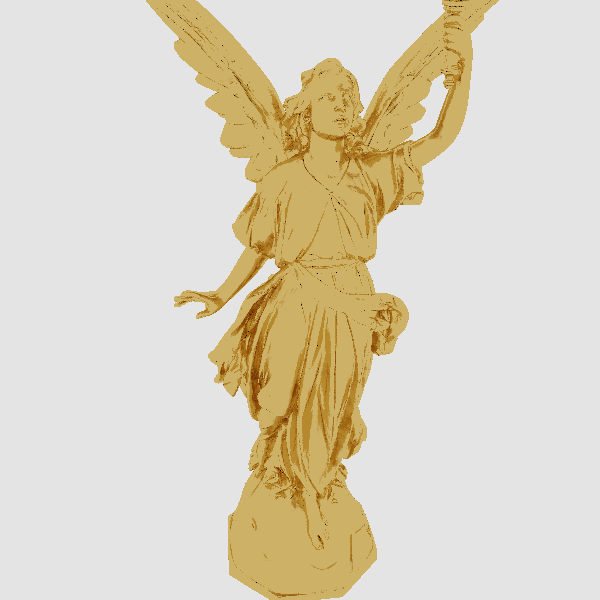
\includegraphics[width=0.8\textwidth]{images/lucy.png}
    \caption{St Lucy statue, rendered with appropriately 2 million triangles}
    \label{fig:Lucy}
\end{figure}
\begin{figure}[!htb]
    \centering
    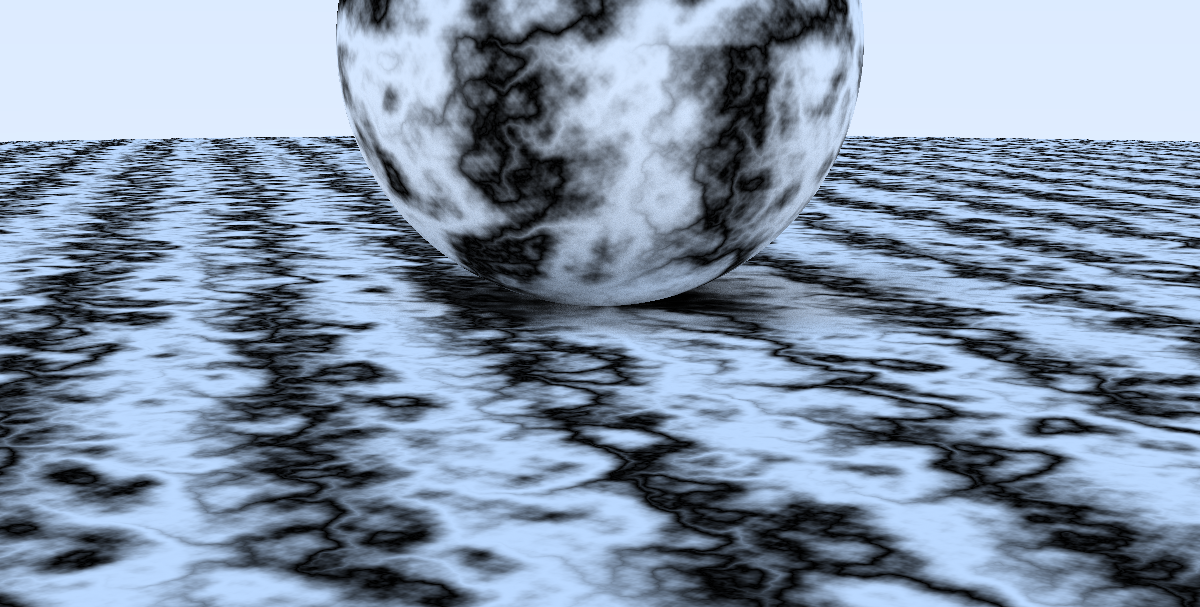
\includegraphics[width=0.8\textwidth]{images/marbling.png}
    \caption{Perlin Noise texture applied to the floor and the sphere}
    \label{fig:Marbling}
\end{figure}
\begin{figure}[h]
    \centering
    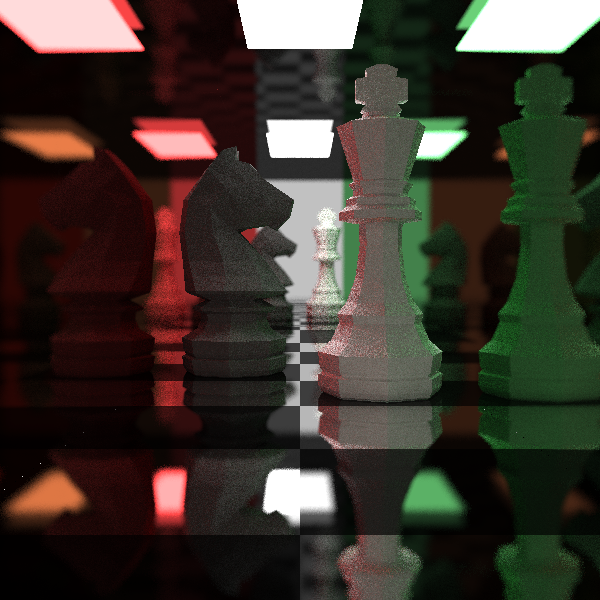
\includegraphics[width=0.8\textwidth]{images/Chess.png}
    \caption{Two chess pieces with reflective walls and mirrors}
    \label{fig:Chess}
\end{figure}
\begin{figure}[h]
    \centering
    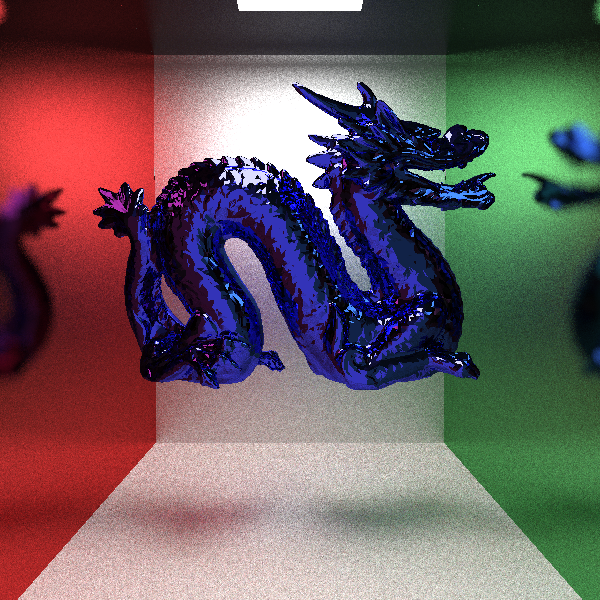
\includegraphics[width=0.8\textwidth]{images/Dragon1.png}
    \caption{A metallic dragon}
    \label{fig:Dragon}
\end{figure}
\begin{figure}[h]
    \centering
    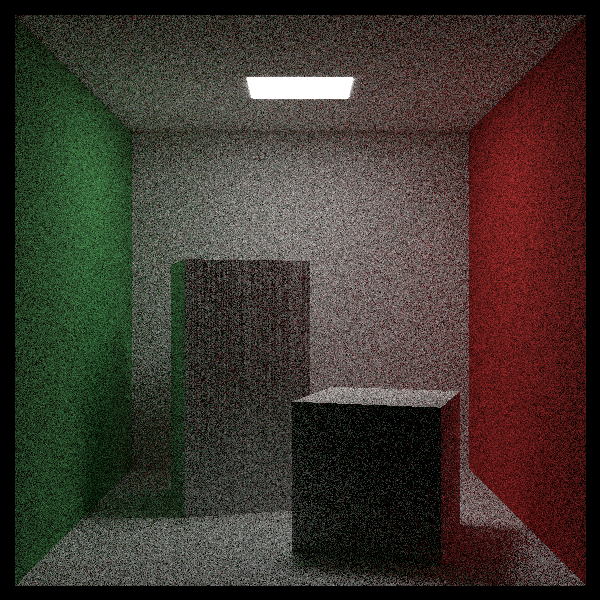
\includegraphics[width=0.8\textwidth]{images/CornellBox.png}
    \caption{A standard Cornell Box}
    \label{fig:CornellBox}

\end{figure}
\end{document}